\documentclass[10pt,xcolor=table ]{beamer}
	
\usetheme{metropolis}
\usepackage{appendixnumberbeamer}

\usepackage{booktabs}
\usepackage[scale=2]{ccicons}

\usepackage{pgfplots}
\usepgfplotslibrary{dateplot}

\usepackage{xspace}
\usepackage{graphicx}
\usepackage{graphics}


\usepackage[spanish]{babel}
\usepackage[utf8]{inputenc}

\usepackage{decorule}
\newcommand{\decoRule}{\rule{\textwidth}{.4pt}} % New command for a rule to be used under figures


\usepackage{pgf-pie}
\usepackage{pgfplots}

\usepackage[export]{adjustbox}


\definecolor{UniBlue}{RGB}{255,255,255}
\setbeamercolor{background canvas}{bg=UniBlue}


\title{Desarrollo de un sistema de gestión de programas de estudio orientado a resultados pedagógicos}
\subtitle{Defensa final de tesis de Ingeniería en Informática}
\author{Luis Fernando Villalba Vera}
\institute{Universidad Católica - Nuestra Señora de la Asunción}
\date{\today}
\titlegraphic{\hfill
\includegraphics[height=1.7cm]{../Figuras/uca}}

\begin{document}

\maketitle

\begin{frame}{Contenido}
	\begin{enumerate}
	    \item Motivación
	    \item Objetivos
	    \item Marco teórico
	    \item Estado del arte
	    \item Propuesta de trabajo
	    \item Proceso de desarrollo
	    \item Validación del desarrollo
	    \item Conclusión y aportes
	 \end{enumerate}
\end{frame}

% JUSTIFICACIÓN
\section{Motivación}
\begin{frame}{Problemática}
  \begin{itemize}[<+- | alert@+>]
    \item Estudiantes con habilidades comprobadas
    \item Evaluación basada en competencias
    \item Sistemas de gestión de evaluaciones (AMS)
    \item Diseño de programas educativos orientados a competencias
    \item Sistemas de gestión curricular (CMS)
  \end{itemize}
\end{frame}

\subsection{Diseño de cursos y programas}
\begin{frame}{Diseño de cursos y programas}
	\begin{figure}
		\centering
	    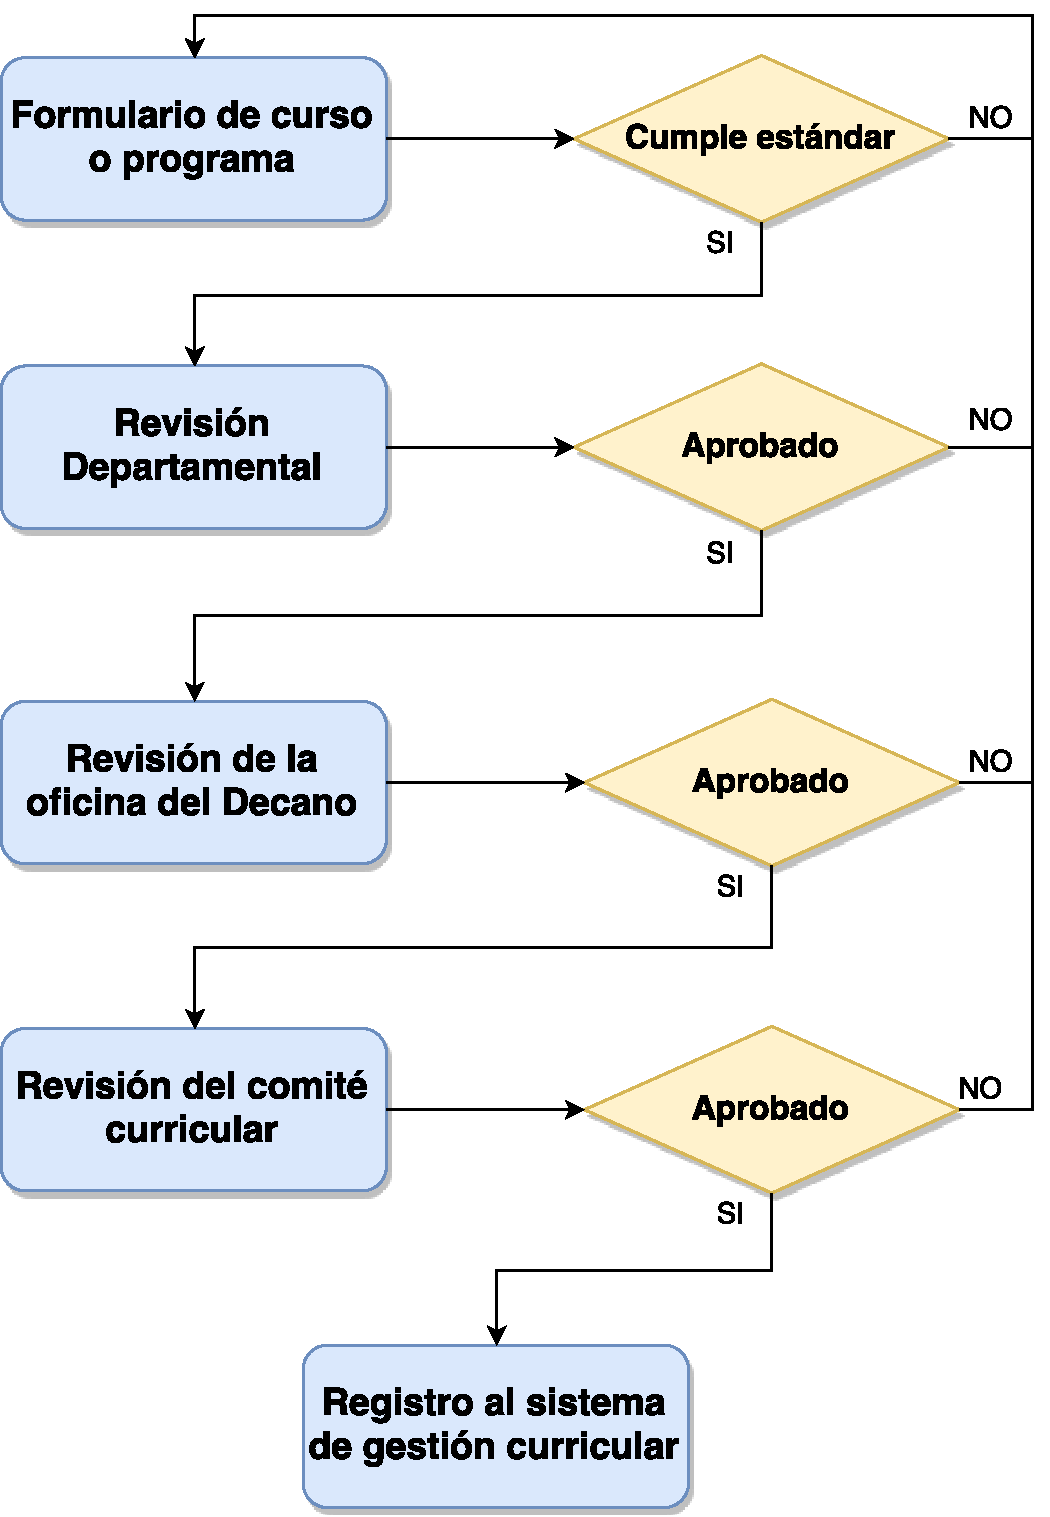
\includegraphics[scale=0.3]{../Figuras/course_creation_flow}
	\end{figure}
\end{frame}

\subsection{Disponibilidad en el sistema de gestión de competencias}
\begin{frame}{Disponibilidad en el sistema de gestión de competencias}
	\begin{figure}
		\centering
	    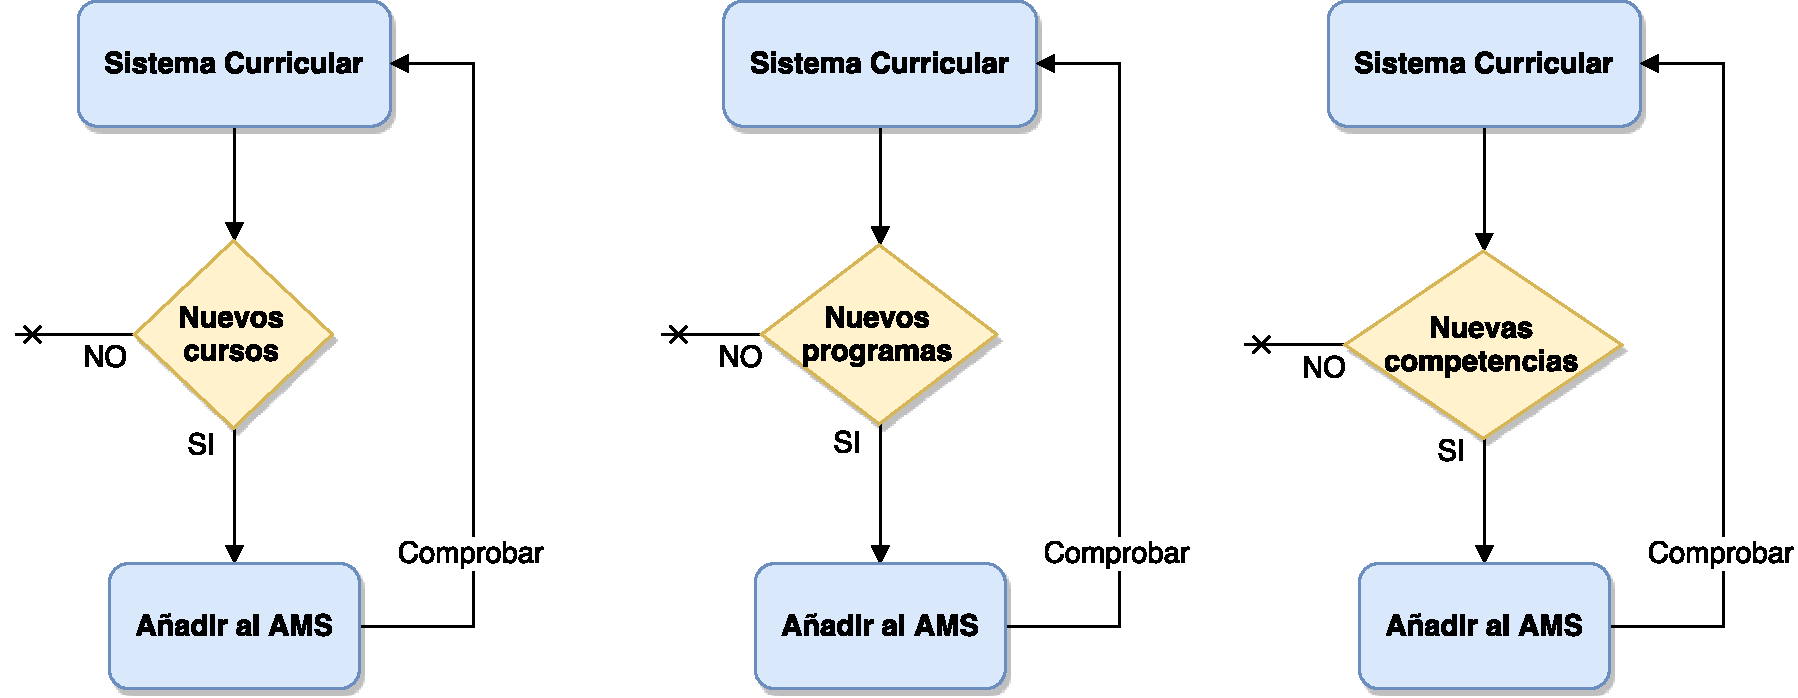
\includegraphics[scale=0.35]{../Figuras/after_creation}
	\end{figure}
\end{frame}

% OBJETIVOS
\section{Objetivos}
\subsection{Objetivos}
\begin{frame}[t]{Objetivos}
	\metroset{block=fill}
	\begin{alertblock}{Objetivo general}
        Diseñar una aplicación que permita integrar y estructurar tareas separadas de un sistema académico para una gestión de programas educativos orientados a resultados pedagógicos, que provea soporte a flujos de trabajo para sus diferentes etapas de aprobación.
      \end{alertblock}

	\metroset{block=fill}
	\begin{alertblock}<2>{Objetivos específicos}
        \begin{itemize}
        	\item Realizar un relevamiento de los requerimientos, diseño e implementación de un sistema de gestión de programas orientado a competencias.
        	\item Realizar el proyecto en un marco de programación ágil, estimando y desarrollando la aplicación de acuerdo a las directrices brindadas por la metodología.
        	\item Validar la herramienta desarrollada: con expertos del dominio principalmente y de manera preliminar con experiencias limitadas con los usuarios finales.
        \end{itemize}
    \end{alertblock}
\end{frame}

% MARCO TEORICO
\section{Marco teórico}
\subsection{Software as a Service}
\begin{frame}{Software as a Service}
	\metroset{block=fill}
	\begin{alertblock}{Definición}
		Paradigma de entrega de software como servicio a través de una red.
	\end{alertblock}

	\begin{columns}[c,onlytextwidth]
    	\column{0.6\textwidth}
		\begin{block}{Características}
			\begin{itemize}
	        	\item Modelo de suscripción.
	        	\item Acceso y administración a través de una red.
	        	\item Actividades gestionadas desde ubicaciones centrales.
	        	\item Actualizaciones centralizadas.
	      		\item Arquitectura multi-tenant.
	    	\end{itemize}
		\end{block}
	    \column{0.4\textwidth}
		\begin{figure}[H]
			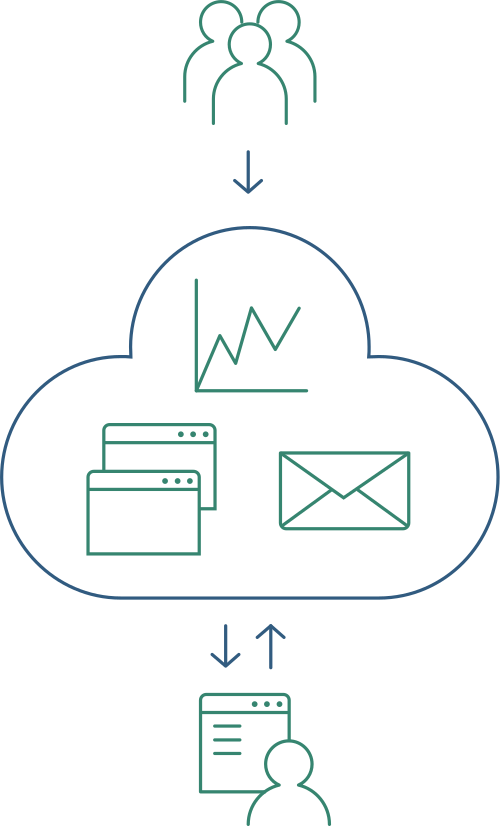
\includegraphics[scale=0.23]{../Figuras/saas}
		\end{figure}
  	\end{columns}
\end{frame}

\subsection{Sistemas de gestión de evaluaciones}
\begin{frame}{Sistemas de gestión de evaluaciones}
	\begin{figure}
		\centering
	    \includegraphics<1>[scale=0.55]{../Figuras/ams_1}
	    \includegraphics<2>[scale=0.55]{../Figuras/ams_2}
	    \includegraphics<3>[scale=0.55]{../Figuras/ams_3}
	\end{figure}
\end{frame}

\subsection{Metodología ágil}
\begin{frame}{Metodología ágil}
	\metroset{block=fill}
	\begin{alertblock}{Definición}
		Enfoque para toma de decisiones basado en el desarrollo iterativo e incremental.
	\end{alertblock}

	\begin{columns}[c,onlytextwidth]
    	\column{0.5\textwidth}
		\begin{block}{Características}
			\begin{itemize}
	        	\item Entregas de valor agregado en iteraciones.
	        	\item Adaptación al cambio.
	        	\item El cliente es parte del proceso de desarrollo.
	    	\end{itemize}
		\end{block}
	    \column{0.5\textwidth}
		\begin{figure}
		    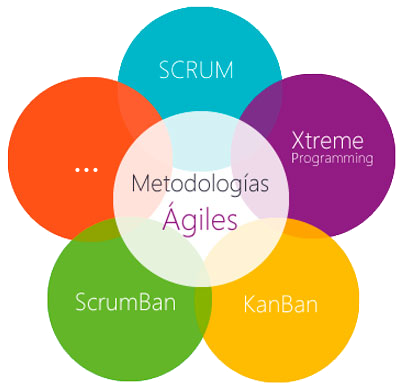
\includegraphics[scale=0.32]{../Figuras/met_agiles}
		\end{figure}
  	\end{columns}
\end{frame}

\subsection{Interacción Humano-Computador}
\begin{frame}{Interacción Humano-Computador}
	\metroset{block=fill}
	\begin{alertblock}{Definición}
		Diseño que busca lograr un balance óptimo entre la calidad y la eficiencia de los servicios.
	\end{alertblock}

	\begin{columns}[c,onlytextwidth]
    	\column{0.6\textwidth}
		\begin{block}{Características}
			\begin{itemize}
	        	\item Definen la funcionalidad y la interacción de los usuarios.
	        	\item Facilita e incrementa la usabilidad de los sistemas.
	        	\item Busca optimizar la interacción y el procesamiento de información.
	    	\end{itemize}
		\end{block}
	    \column{0.4\textwidth}
		\begin{figure}
		    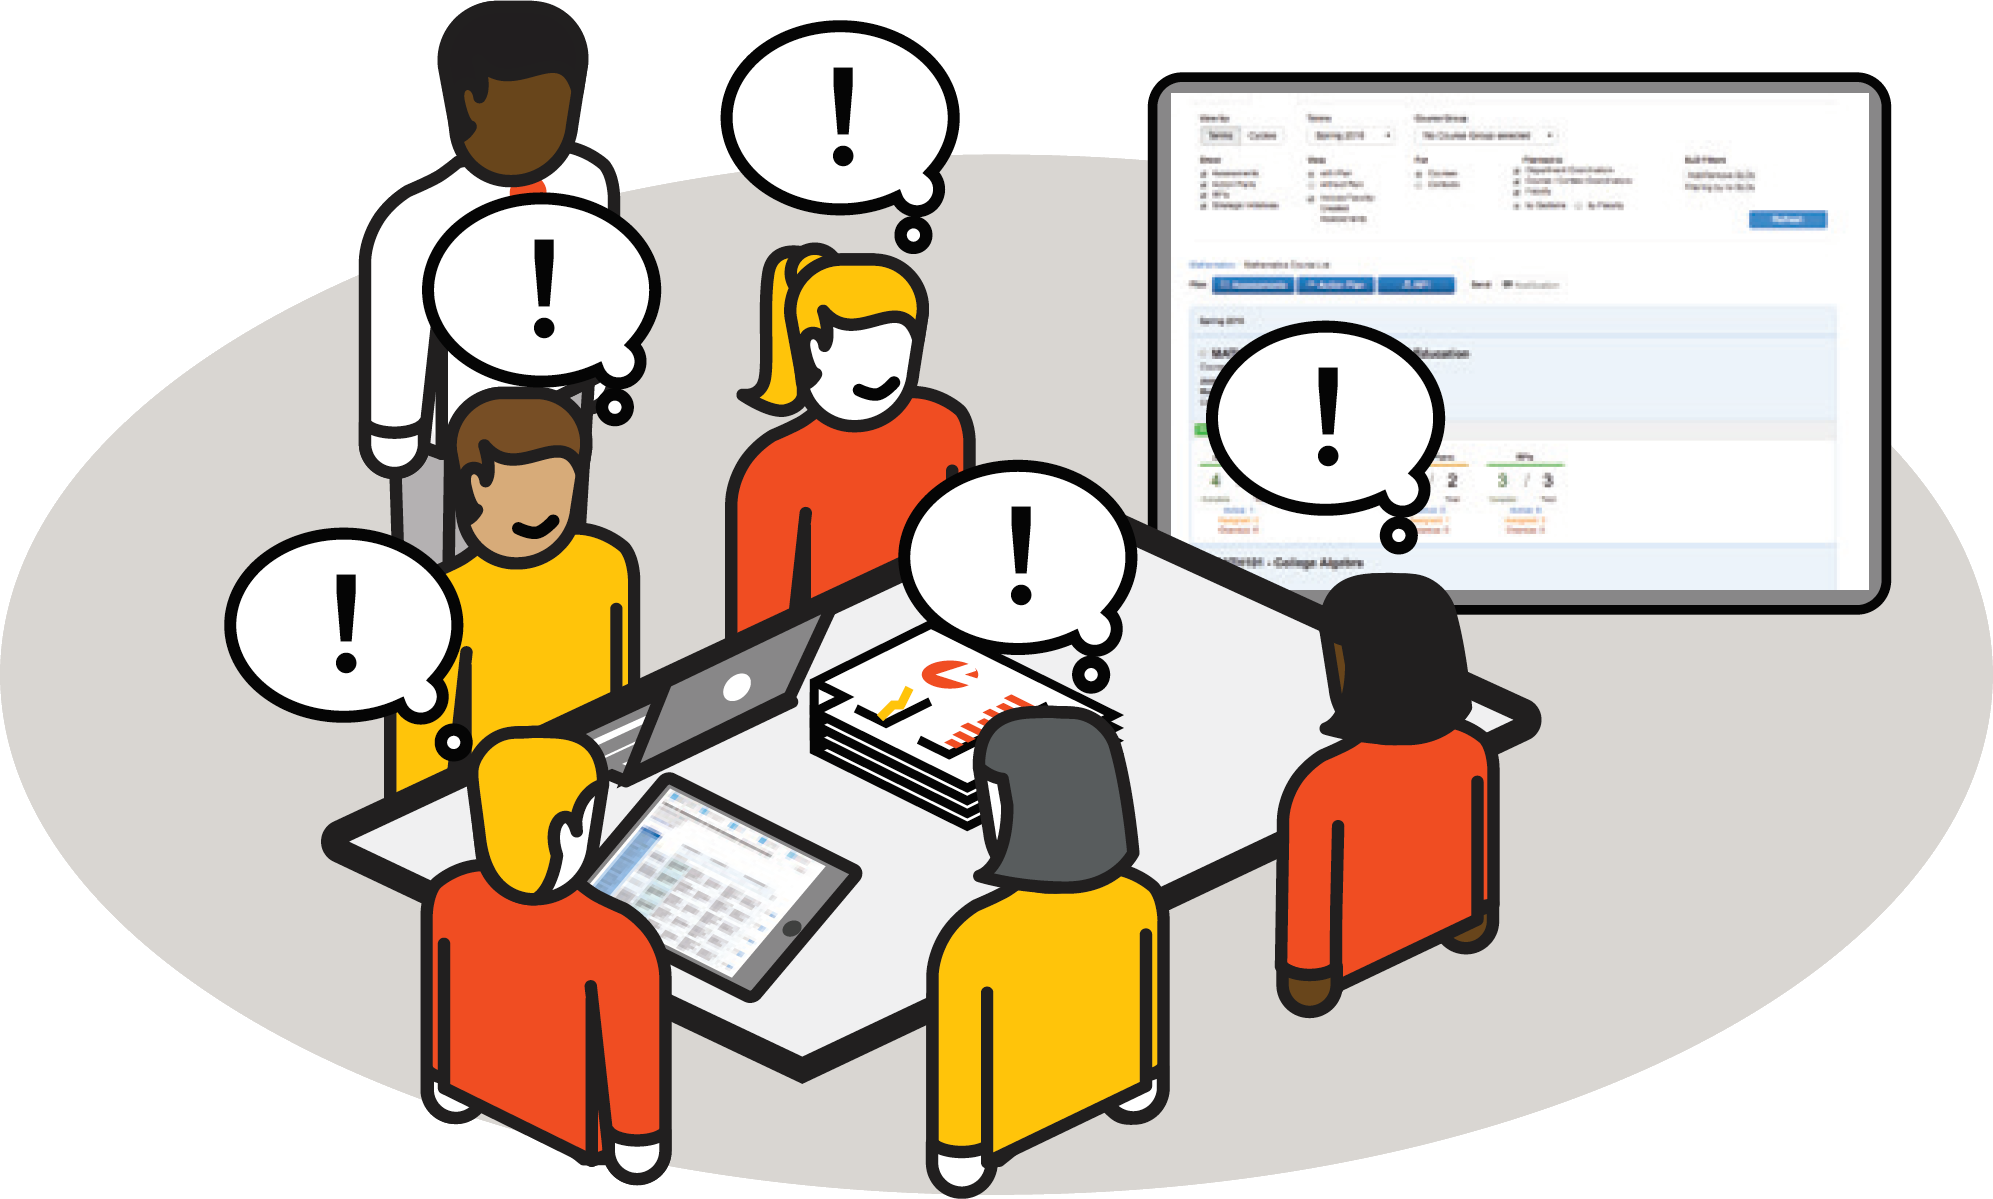
\includegraphics[scale=0.12]{../Figuras/happy_agile}
		\end{figure}
  	\end{columns}
\end{frame}

% ESTADO DEL ARTE
\section{Estado del arte}
\subsection{Sistemas de gestión curricular}
\begin{frame}{Sistemas de gestión curricular}
	\begin{figure}
		\centering
	    
\includegraphics[scale=0.5]{../Figuras/cms_alternatives}
	\end{figure}
\end{frame}

\subsection{Comparación de sistemas relacionados}
\begin{frame}{Comparación de sistemas relacionados}
  	\begin{table}[H]
  	\small
	\centering
	\resizebox{\columnwidth}{!}{%
		\begin{tabular}{lllccl}
		\toprule
		\multicolumn{3}{l}{Características}                                                & CurricUNET                       & CourseLeaf            & DECA         \\
		\midrule
		\rowcolor[HTML]{ECF4FF}
		\multicolumn{3}{l}{Creación y versionamiento de competencias.}                     &                                  &                       &              \\
		\multicolumn{3}{l}{Creación y versionamiento de cursos.}                           & $\checkmark$                     & $\checkmark$          & $\checkmark$ \\
		\multicolumn{3}{l}{Creación y versionamiento de programas de estudio.}             & $\checkmark$                     & $\checkmark$          &              \\
		\multicolumn{3}{l}{Cumple los Estándares de códigos de California.} 			   & $\checkmark$                     &                       &              \\
		\rowcolor[HTML]{ECF4FF}
		\multicolumn{3}{l}{Historial de versiones de competencias.}     			       & 			                      & 		              &  			 \\
		\multicolumn{3}{l}{Historial de versiones de cursos.}     			               & $\checkmark$                     & $\checkmark$          & $\checkmark$ \\
		\multicolumn{3}{l}{Historial de versiones de programas de estudio.}     		   & $\checkmark$                     &  			          & 			 \\
		\multicolumn{3}{l}{Reporte de Comparación entre versiones de cursos.}              & 			                      &                       & $\checkmark$ \\
		\rowcolor[HTML]{ECF4FF}
		\multicolumn{3}{l}{Soporta competencias de aprendizaje del estudiante.}            &                      			  &                       &              \\
		\multicolumn{3}{l}{Plantilla de flujo de trabajo customizable.}                    & $\checkmark$                     &                       &              \\
		\multicolumn{3}{l}{Permite asignar roles evaluadores en la aplicación.}            & $\checkmark$                     & $\checkmark$          &              \\
		\multicolumn{3}{l}{Permite asignar usuarios como colaboradores.}                   & $\checkmark$                     &                       &              \\
		\multicolumn{3}{l}{Soporte de correlatividades entre cursos.}                      & $\checkmark$ 					  &						  &              \\
		\multicolumn{3}{l}{Incluye un catálogo de cursos.}                   		   	   & $\checkmark$					  &	$\checkmark$		  & $\checkmark$ \\
		\multicolumn{3}{l}{Incluye un catálogo de programas de estudio.}                   & $\checkmark$					  &	            		  &              \\
		\rowcolor[HTML]{ECF4FF}
		\multicolumn{3}{l}{Incluye un catálogo de competencias.}                   	       & 								  &						  & 			 \\
		\multicolumn{3}{l}{UX intuitiva y efectiva.}     			   					   &                                  & $\checkmark$          & $\checkmark$ \\
		\bottomrule
		\end{tabular}
	}
	\end{table}
\end{frame}

% PROPUESTA DE TRABAJO
\section{Propuesta de trabajo}
\subsection{Definición del proyecto}
\begin{frame}{Caso de estudio}
	\metroset{block=fill}
	\begin{alertblock}{Definición}
		Desarrollo de un sistema de gestión de cursos y programas orientado a competencias con un enfoque HCI y observación participante.
	\end{alertblock}

	\begin{block}<2>{Características}
		\begin{itemize}
			\item Arquitectura Software as a Service.
			\item Utilización de abordaje ágil de desarrollo.
        	\item Observación participante como método de recolección de información.
        	\item HCI para mejorar la usabilidad e interacción con el usuario.
			\item Validaciones por un equipo de expertos en dominio educativo.
    	\end{itemize}
	\end{block}
\end{frame}

\subsection{Módulo de gestión curricular integrado a un AMS}
\begin{frame}{Módulo de gestión curricular integrado a un AMS}
	\begin{figure}
		\centering
	    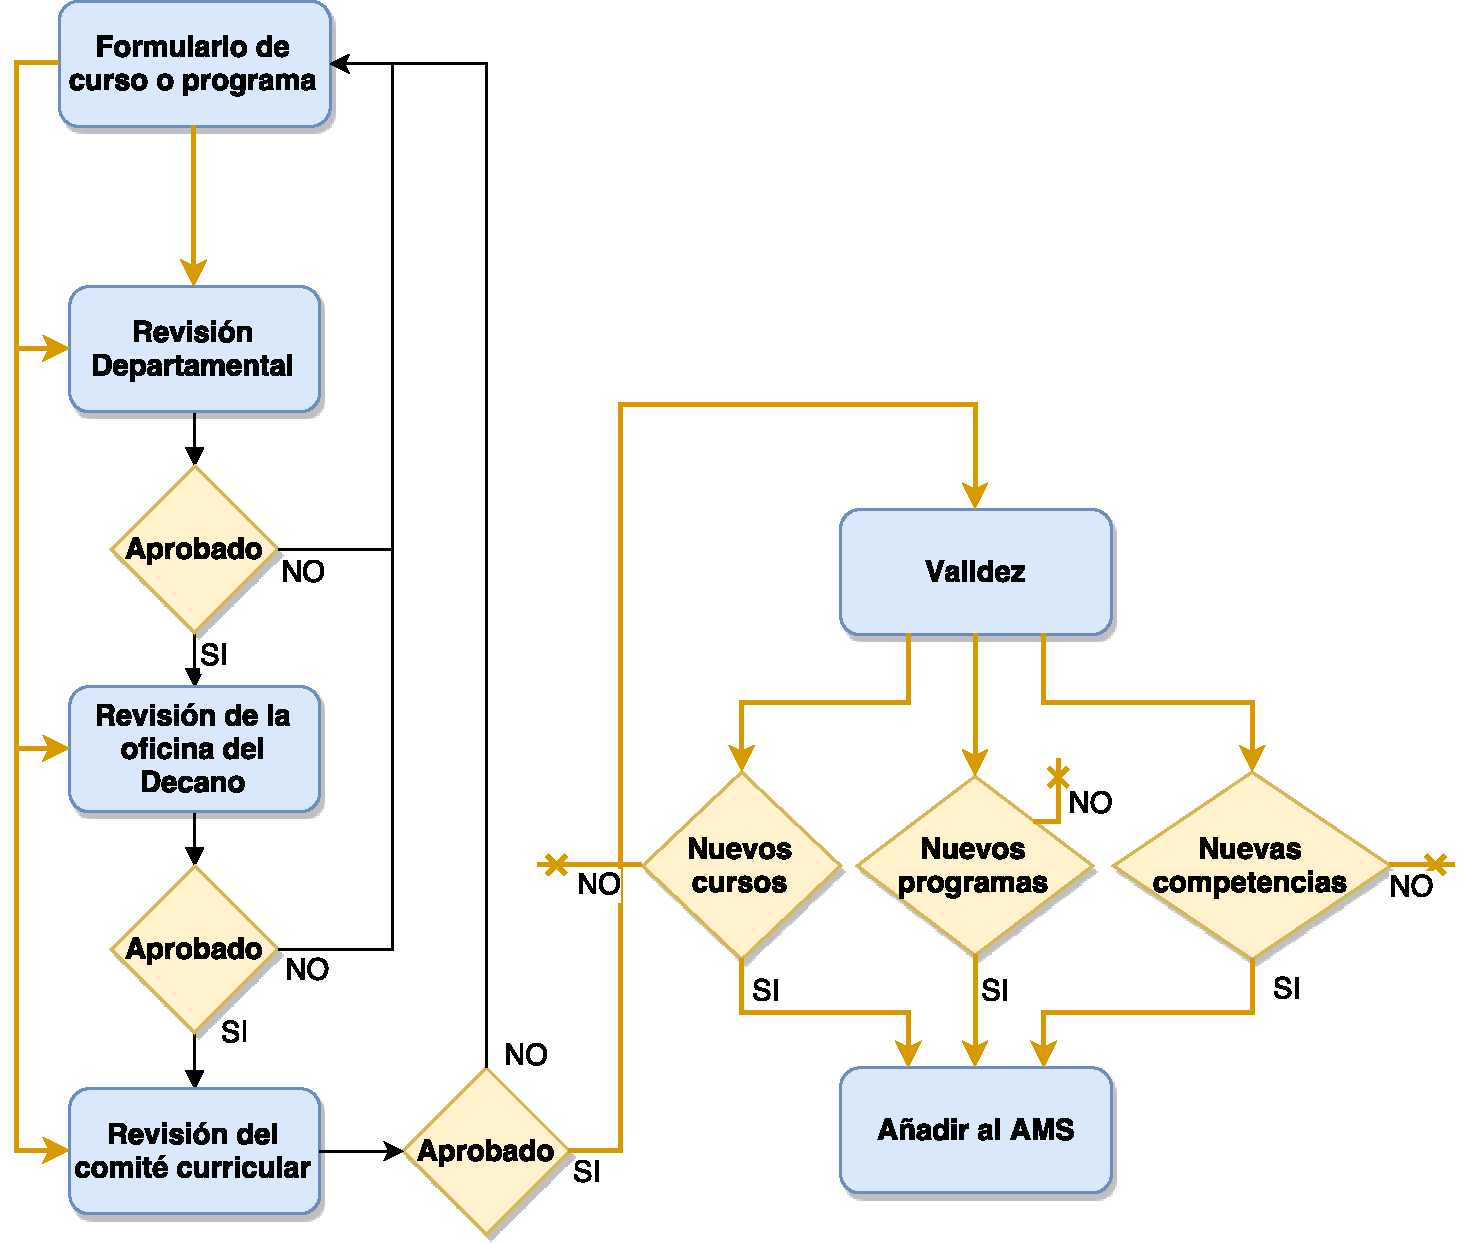
\includegraphics[scale=0.35]{../Figuras/proposal}
	\end{figure}
\end{frame}


\begin{frame}{Modelo de la propuesta de solución}
	\begin{figure}
		\centering
	    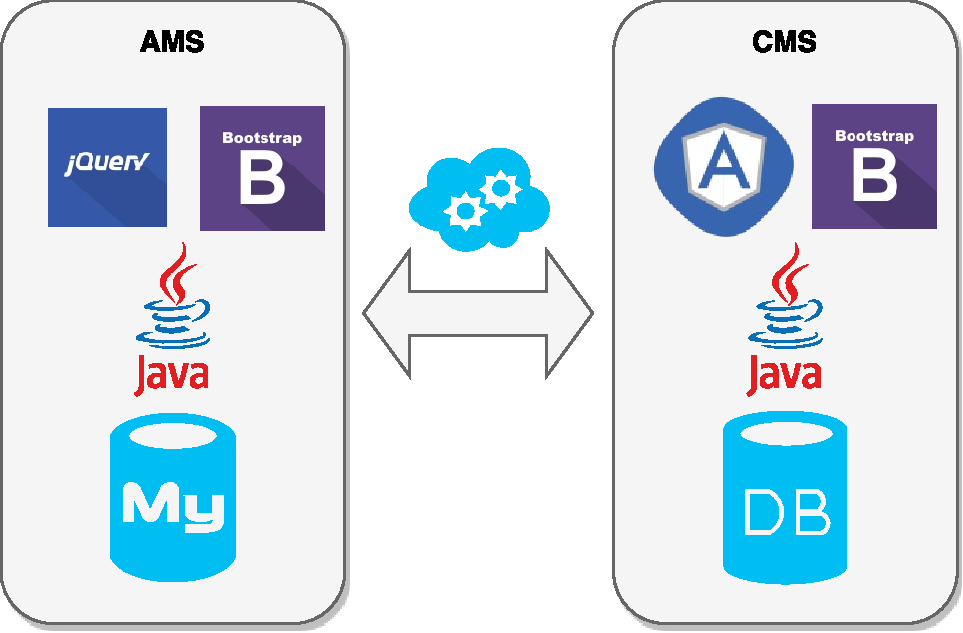
\includegraphics[scale=0.55]{../Figuras/architecture}
	\end{figure}
\end{frame}

% PROCESO DE DESARROLLO
\section{Proceso de desarrollo}
\subsection{Épicas e historias de usuario}
\begin{frame}{Épicas e historias de usuario}
	\begin{figure}
		\centering
	    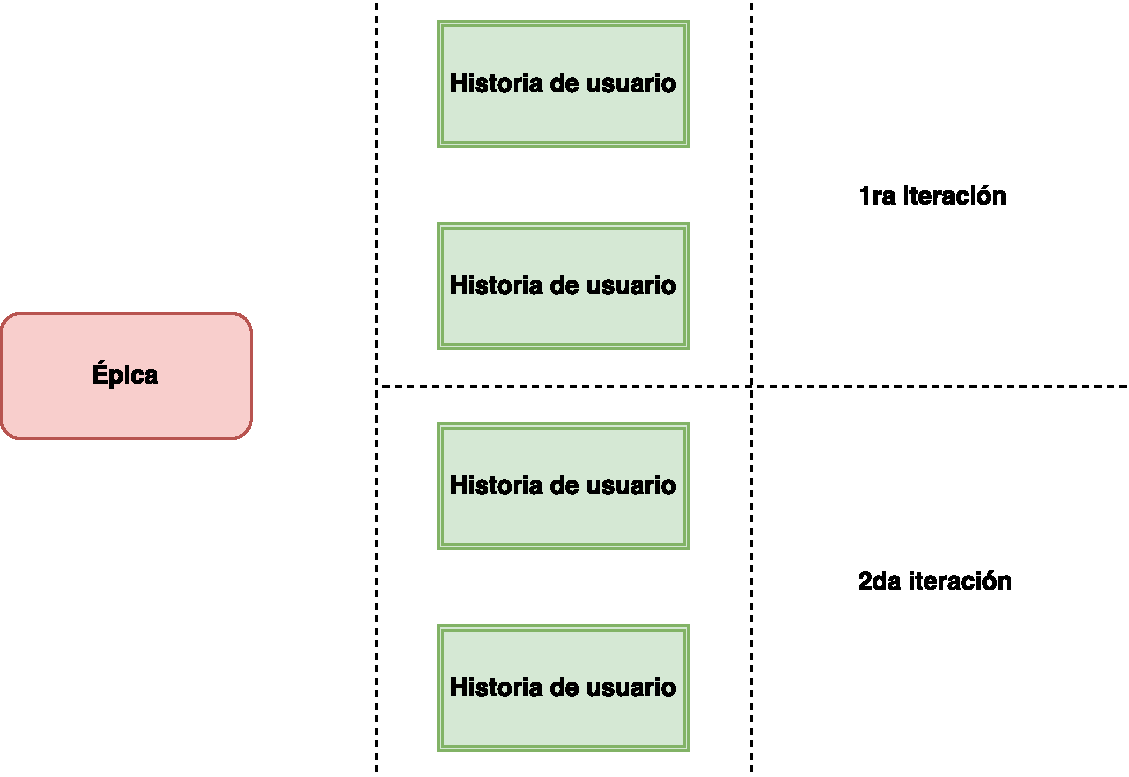
\includegraphics[scale=0.5]{../Figuras/epic_diagram}
	\end{figure}
\end{frame}

\subsection{Flujo de la iteración}
\begin{frame}{Flujo de la iteración}
	\begin{figure}
		\centering
		\includegraphics<1>[scale=0.235]{../Figuras/flujo_scrum_1}
		\includegraphics<2>[scale=0.235]{../Figuras/flujo_scrum_2}
		\includegraphics<3>[scale=0.235]{../Figuras/flujo_scrum_3}
		\includegraphics<4>[scale=0.235]{../Figuras/flujo_scrum_4}
		\includegraphics<5>[scale=0.235]{../Figuras/flujo_scrum_5}
	\end{figure}
	\decoRule \\
  	\tiny \textit{Charles G Cobb. The project manager’s guide to mastering Agile: Principles and practices for an adaptive approach. John Wiley \& Sons, 2015.} \\
\end{frame}

\section{Funcionalidades del módulo curricular}
\subsection{Definición de plantillas}
\begin{frame}{Definición de plantillas}
\begin{figure}
		\centering
	    \includegraphics<1>[scale=0.55]{../Figuras/Pantallas/funcionalidades_1}
	    \includegraphics<2>[scale=0.55]{../Figuras/Pantallas/funcionalidades_2}
	\end{figure}
\end{frame}

\begin{frame}{Plantillas de flujos de trabajo}
	\begin{figure}
		\centering
		\includegraphics<1>[scale=0.4]{../Figuras/Pantallas/template_1}
		\includegraphics<2>[scale=0.3]{../Figuras/Pantallas/template_2}
		\includegraphics<3>[scale=0.3]{../Figuras/Pantallas/template_3}
	\end{figure}
\end{frame}


\subsection{Utilización de flujos de trabajo}
\begin{frame}{Utilización de flujos de trabajo}
\begin{figure}
		\centering
	    \includegraphics<1>[scale=0.55]{../Figuras/Pantallas/funcionalidades_2}
	    \includegraphics<2>[scale=0.55]{../Figuras/Pantallas/funcionalidades_3}
	\end{figure}
\end{frame}

\begin{frame}{Flujo de trabajo para cursos}
	\begin{figure}
		\centering
		\includegraphics<1>[scale=0.275]{../Figuras/Pantallas/course_creation_1}
		\includegraphics<2>[scale=0.3]{../Figuras/Pantallas/course_creation_7}
		\includegraphics<3>[scale=0.3]{../Figuras/Pantallas/course_creation_submit}
		\includegraphics<4>[scale=0.27]{../Figuras/Pantallas/course_revision_1}
		\includegraphics<5>[scale=0.3]{../Figuras/Pantallas/course_revision_4}
	\end{figure}
\end{frame}


\subsection{Lista de cursos, programas y competencias}
\begin{frame}{Lista de cursos, programas y competencias}
\begin{figure}
		\centering
	    \includegraphics<1>[scale=0.55]{../Figuras/Pantallas/funcionalidades_3}
	    \includegraphics<2>[scale=0.55]{../Figuras/Pantallas/funcionalidades_4}
	\end{figure}
\end{frame}

\begin{frame}{Catálogo de cursos, programas y competencias}
	\begin{figure}
		\centering
		\includegraphics<1>[scale=0.3]{../Figuras/Pantallas/curriculum_list_1}
		\includegraphics<2>[scale=0.3]{../Figuras/Pantallas/curriculum_list_2}
		\includegraphics<3>[scale=0.25]{../Figuras/Pantallas/curriculum_list_3}
		\includegraphics<4>[scale=0.3]{../Figuras/Pantallas/curriculum_list_4}
	\end{figure}
\end{frame}


\subsection{Buzón de entradas}
\begin{frame}{Buzón de entradas}
\begin{figure}
		\centering
	    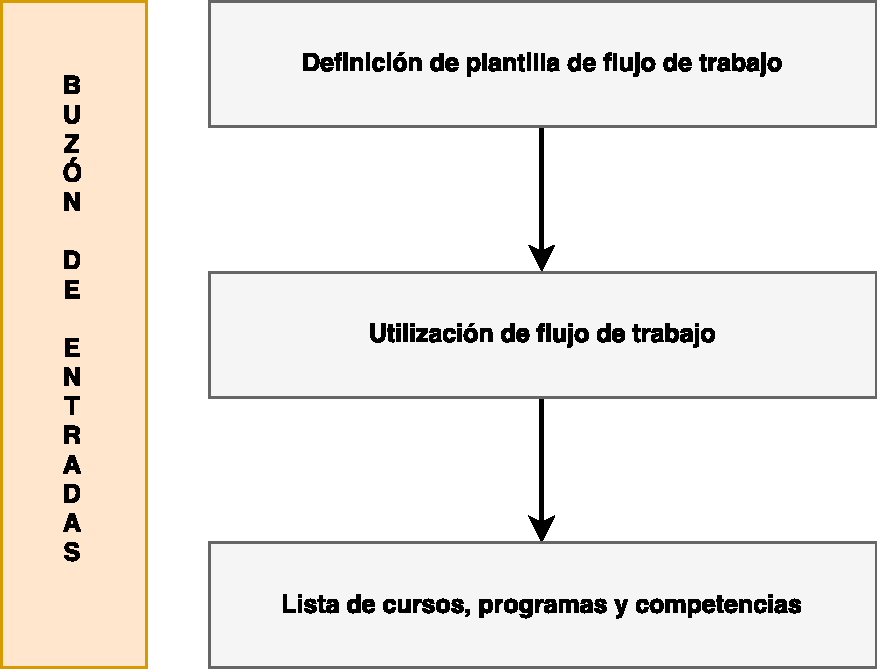
\includegraphics[scale=0.55]{../Figuras/Pantallas/funcionalidades_1}
	\end{figure}
\end{frame}

\begin{frame}{Buzón de entradas}
	\begin{figure}
		\centering
		\includegraphics<1>[scale=0.3]{../Figuras/Pantallas/inbox}
		\includegraphics<2>[scale=0.3]{../Figuras/Pantallas/inbox_2}
	\end{figure}
\end{frame}

\subsection{Resultados}
\begin{frame}{Resultados}
	\begin{figure}
		\centering
	    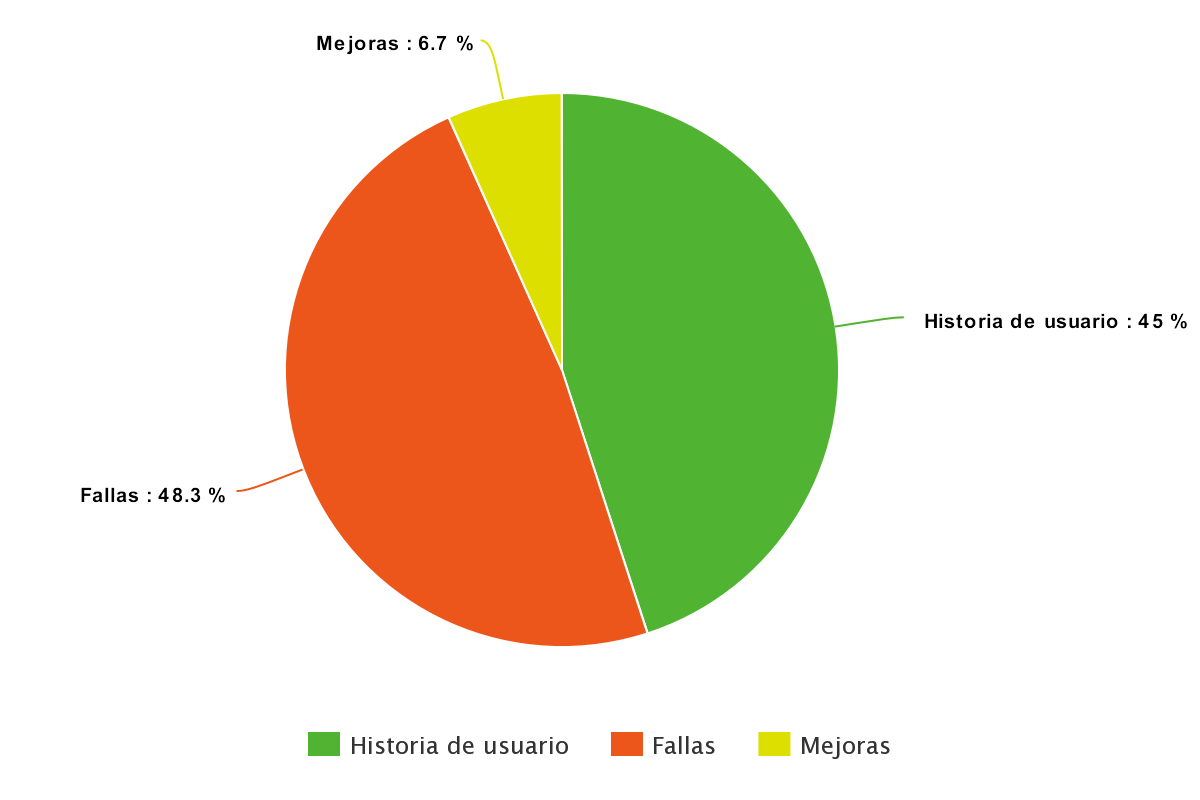
\includegraphics[scale=0.235]{../Figuras/tickets_tipo}
	\end{figure}
\end{frame}

\begin{frame}{Resultados}
	\begin{figure}
		\centering
	    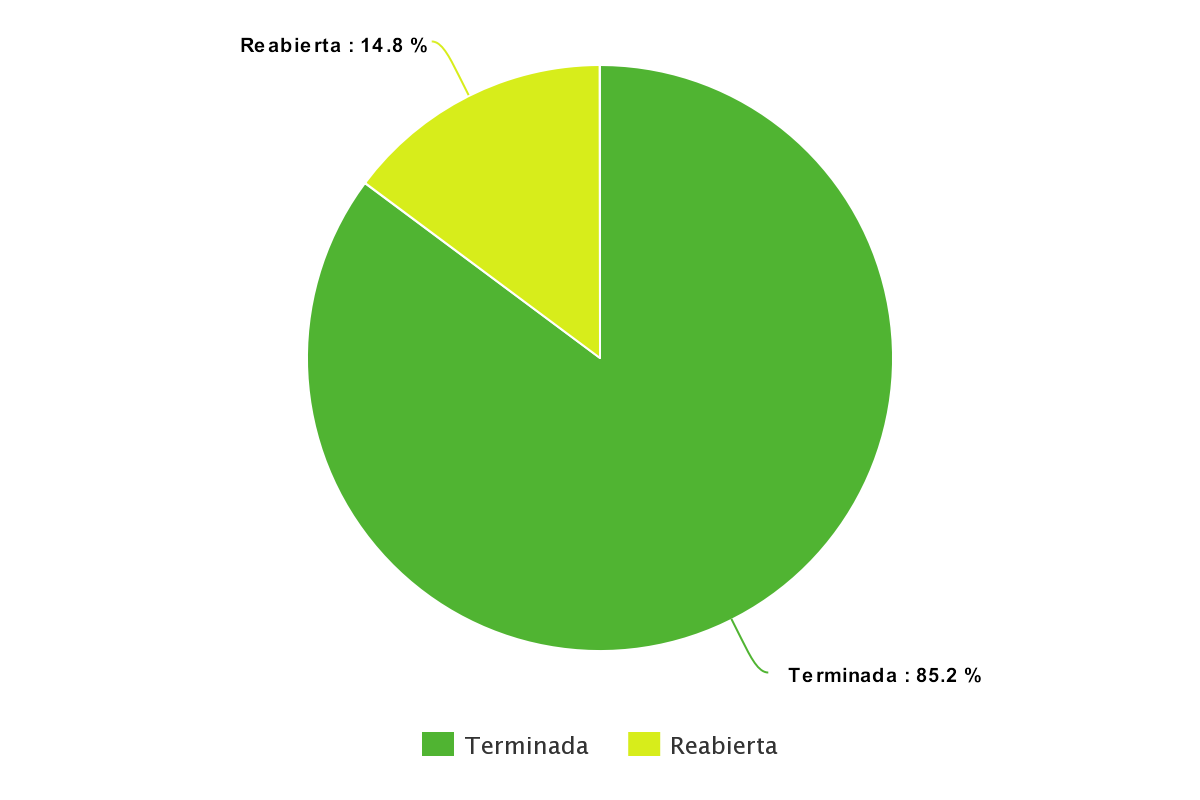
\includegraphics[scale=0.235]{../Figuras/historias_cerradas_reabiertas}
	\end{figure}
\end{frame}

% VALIDACIÓN DEL DESARROLLO
\section{Validación del desarrollo}
\subsection{Por parte de los programadores}
\begin{frame}{Por parte de los programadores}
	\begin{itemize}[<+- | alert@+>]
		\item Pull Request
	    \item Revisión de códigos
	    \item Pruebas manuales y automatizadas
	    \item Comprobación de los criterios de aceptación
	\end{itemize}
\end{frame}

\subsection{Por parte de los expertos en dominio}
\begin{frame}{Por parte de los expertos en dominio}
	\begin{figure}
		\centering
	    \includegraphics<1>[scale=0.35]{../Figuras/workflow_1}
	    \includegraphics<2>[scale=0.35]{../Figuras/workflow_2}
	    \includegraphics<3>[scale=0.35]{../Figuras/workflow_3}
	    \includegraphics<4>[scale=0.35]{../Figuras/workflow_4}
	\end{figure}
\end{frame}


% CONCLUSIÓN Y APORTES
\section{Conclusión y aportes}
\subsection{Conclusión}
\begin{frame}{Funcionalidades del módulo curricular}
	\begin{table}[]
	\small
	\centering
	\resizebox{\columnwidth}{!}{%
	\begin{tabular}{@{}lllccll@{}}
	\midrule
	\multicolumn{3}{l}{Características}                                     & CurricUNET   & CourseLeaf   & DECA         & MC           \\ \midrule
	\rowcolor[HTML]{ECF4FF}
	\multicolumn{3}{l}{Creación y versionamiento de competencias.}          &              &              &              & $\checkmark$ \\
	\multicolumn{3}{l}{Creación y versionamiento de cursos.}                & $\checkmark$ & $\checkmark$ & $\checkmark$ & $\checkmark$ \\
	\multicolumn{3}{l}{Creación y versionamiento de programas de estudio.}  & $\checkmark$ & $\checkmark$ &              & $\checkmark$ \\
	\multicolumn{3}{l}{Cumple los Estándares de códigos de California.}     & $\checkmark$ &              &              & $\checkmark$ \\
	\rowcolor[HTML]{ECF4FF}
	\multicolumn{3}{l}{Historial de versiones de competencias.}             &              &              &              & $\checkmark$ \\
	\multicolumn{3}{l}{Historial de versiones de cursos.}                   & $\checkmark$ & $\checkmark$ & $\checkmark$ & $\checkmark$ \\
	\multicolumn{3}{l}{Historial de versiones de programas de estudio.}     & $\checkmark$ &              &              & $\checkmark$ \\
	\multicolumn{3}{l}{Reporte de Comparación entre versiones de cursos.}   &              &              & $\checkmark$ & $\checkmark$ \\
	\rowcolor[HTML]{ECF4FF}
	\multicolumn{3}{l}{Soporta competencias de aprendizaje.}                &              &              &              & $\checkmark$ \\
	\multicolumn{3}{l}{Plantilla de flujo de trabajo customizable.}         & $\checkmark$ &              &              & $\checkmark$ \\
	\multicolumn{3}{l}{Permite asignar roles evaluadores en la aplicación.} & $\checkmark$ & $\checkmark$ &              & $\checkmark$ \\
	\multicolumn{3}{l}{Permite asignar usuarios como colaboradores.}        & $\checkmark$ &              &              & $\checkmark$ \\
	\multicolumn{3}{l}{Soporte de correlatividades entre cursos.}           & $\checkmark$ &              &              & $\checkmark$ \\
	\multicolumn{3}{l}{Incluye un catálogo de cursos.}                      & $\checkmark$ & $\checkmark$ & $\checkmark$ & $\checkmark$ \\
	\multicolumn{3}{l}{Incluye un catálogo de programas de estudio.}        & $\checkmark$ &              &              & $\checkmark$ \\
	\rowcolor[HTML]{ECF4FF}
	\multicolumn{3}{l}{Incluye un catálogo de competencias.}                &              &              &              & $\checkmark$ \\
	\multicolumn{3}{l}{UX intuitiva y efectiva.}                            &              & $\checkmark$ & $\checkmark$ & $\checkmark$ \\ \midrule
	\end{tabular}
	}
\end{table}
\end{frame}

\begin{frame}{Conclusiones}
	\metroset{block=fill}
	\begin{alertblock}{Resultados}
		\begin{itemize}
			\item Utilización de la metodología Ágil de desarrollo.
			\item Utilización del motor de base de datos.
			\item Aprobación por parte de los usuarios finales.
			\item Feedback de parte de los usuarios finales.
		\end{itemize}
	\end{alertblock}
\end{frame}

\begin{frame}{Aportes del proyecto}
	\begin{itemize}
	    \item Gestión del diseño y validación de material curricular en el estado de California.
	    \item Reemplaza la preparación manual de formularios, los procesos de revisión y aprobación curricular.
	    \item Permite a las personas trabajar en conjunto sin necesidad de agendar reuniones.
	    \item Permite almacenar datos nuevos, históricos, propuestos y activos de competencias, cursos, y programas.
	    \item Proveer notificaciones automatizadas cuando hay cambios de estado en los flujos de trabajo.
	    \item Según expertos y usuarios, la utilización del módulo desarrollado reduce el tiempo promedio de formulación y revisión de cada flujo de diseño e implementación de flujos de trabajo.
	\end{itemize}
\end{frame}

\begin{frame}{Trabajos futuros}
	\metroset{block=fill}
	\begin{alertblock}{Épicas}
		\begin{itemize}
			\item Importador de cursos
		    \item Migración de motor de base de datos de los flujos de trabajo
		    \item Accesso de información a través de API pública
		    \item Catálogo de cursos
		    \item Flujo de trabajo para evaluaciones
    	\end{itemize}
	\end{alertblock}
\end{frame}

\begin{frame}[standout]
  ¡Gracias por su atención!
\end{frame}


\end{document}
